\documentclass[10pt]{beamer} 
%\usefonttheme{structuresmallcapsserif} 
%% \usepackage{beamerthemeshadow}
\usepackage{verbatim} 
\usetheme{Singapore}
%\usetheme{Pittsburgh}
%\usetheme{Montpellier}
\usepackage{colortbl}
%\usepackage{synttree}
\usepackage{parsetree}
\usepackage{graphicx}
\usepackage{tabularx}
\usepackage[utf8]{inputenc}
\usepackage{listings}
\usepackage{cancel}
\setbeamercolor{alerted text}{fg=lightgray,bg=white}
 \renewcommand{\baselinestretch}{1.5}
     \normalsize
     
% THIS SHOULD BE HERE!
% No unimportant, irrelevant things. Only information.
% Only code if it is of significance.

% get inspired by:
% Simon Jones, Microsoft research, videos.
% John Hughes article How to give a good research presentation.
\title{Towards a Wide-Coverage Grammar for Swedish Using GF}
%\subtitle{\large }
\author{Malin Ahlberg}
\date{}

\begin{document}
\maketitle

 \begin{frame}
  \frametitle{Grammatical Framework}
  \framesubtitle{Introduction}
  A grammar formalism for multilingual applications\\
  \pause
  \vspace{5mm}
  A functional programming language  based on Martin-Löf type theory\\
 \end{frame}


\begin{frame}[containsverbatim]
  \frametitle{Grammatical Framework}
  \verb|PredVP : NP -> VP -> S|\\
  Abstract syntax\\
  %\pause PDF stupid
  \vspace{5mm}
  \verb|PredVP np vp = np ++ vp |\\
  Concrete syntax
 \end{frame}


 \begin{frame}
  \frametitle{Grammatical Framework}
  \framesubtitle{Resource grammars}
  The resource grammars covers about 20 languages \\
  \vspace{5mm}
  \pause
  Extra module for language specific constructions
 \end{frame}

\begin{frame}
  \frametitle{Grammatical Framework}
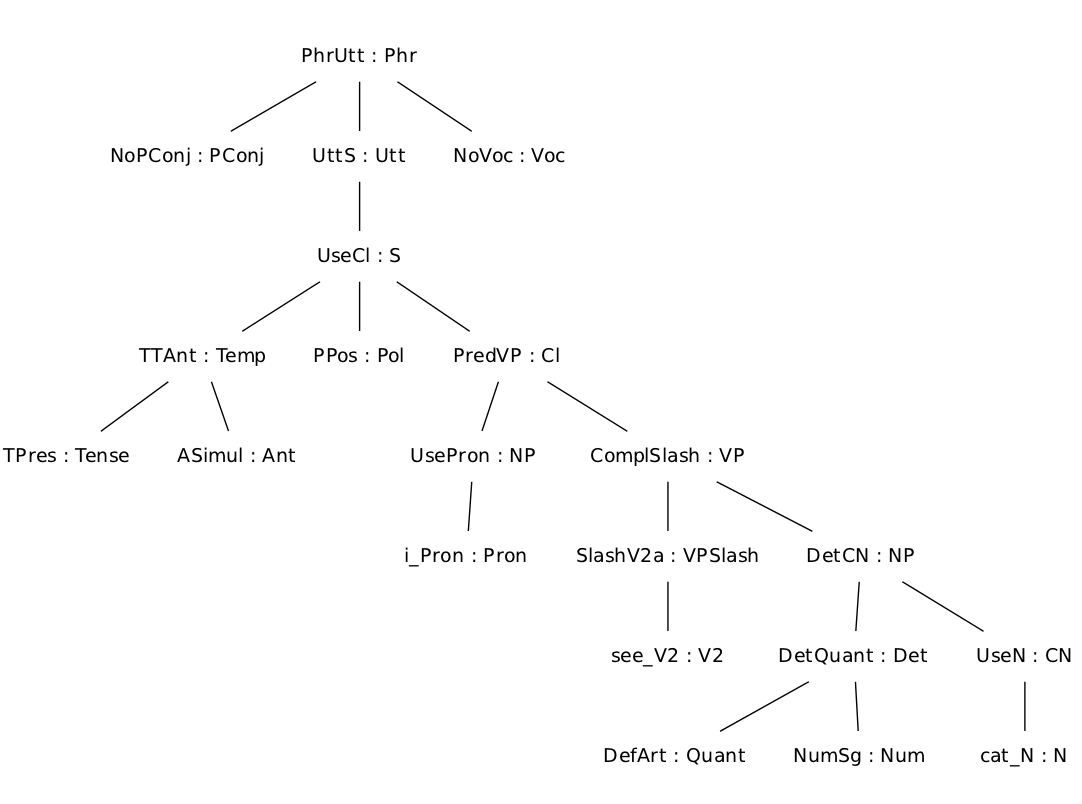
\includegraphics[width=50mm,height=70mm]{gfTree.png}
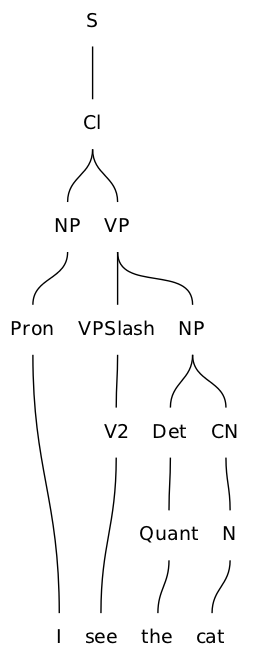
\includegraphics[width=30mm]{gfETree.png}
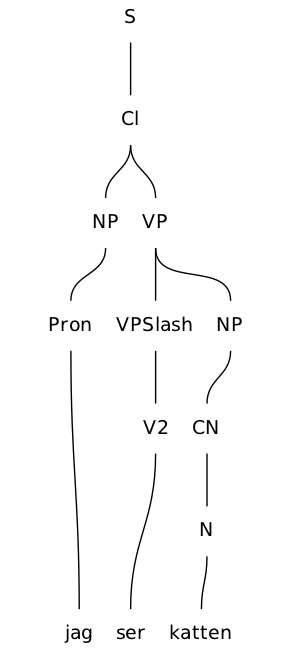
\includegraphics[width=30mm]{gfSTree.png}
 \end{frame}


\begin{frame}
\frametitle{The project}
\framesubtitle{Aims} 
\begin{itemize}
\item{A large-scale lexicon}
\item{A GF treebank}
\item{An extended grammar}
\end{itemize}
\end{frame}

\begin{frame}[containsverbatim]
\frametitle{The project}
\framesubtitle{Talbanken} 
{$\sim$ 6000 manually tagged sentences}
\vspace{5mm}
\begin{tabular}[t]{@{}*{2}{l@{\ }}}
{\begin{parsetree}
\ptbegtree
\ptbeg \ptnode{S} 
\ptbeg \ptnode{SS} \ptbeg \ptnode{NNDDHH}  \ptleaf{Motståndarna} \ptend \ptend
\ptbeg \ptnode{FV} \ptbeg \ptnode{AVPS}  \ptleaf{är} \ptend \ptend
\ptbeg \ptnode{SP} \ptbeg \ptnode{AJ}  \ptleaf{rädda} \ptend \ptend
%\ptbeg \ptnode{OA} 
%    \ptbeg \ptnode{PP} \ptbeg \ptnode{PR} \ptbeg \ptnode{PR} \ptleaf{för} \ptend \ptend
%                       \ptbeg \ptnode{HD} \ptbeg \ptnode{NN} \ptleaf{hundar} \ptend \ptend \ptend \ptend
\ptend
\end{parsetree}}
&
\hspace{-10mm}
{\begin{parsetree}
\ptbegtree
\ptbeg \ptnode{S} 
\ptbeg \ptnode{SS} \ptbeg \ptnode{NNDDHH}  \ptleaf{Motståndarna} \ptend \ptend
\ptbeg \ptnode{FV} \ptbeg \ptnode{AVPS}  \ptleaf{är} \ptend \ptend
\ptbeg \ptnode{SP} \ptbeg \ptnode{AJ}  \ptleaf{rädda} \ptend \ptend
%\ptbeg \ptnode{OA} 
%    \ptbeg \ptnode{PP} \ptbeg \ptnode{PR} \ptbeg \ptnode{PR} \ptleaf{för} \ptend \ptend
%                       \ptbeg \ptnode{HD} \ptbeg \ptnode{NN} \ptleaf{hundar} \ptend \ptend \ptend \ptend
\ptend
\end{parsetree}}\\
\end{tabular}


%\item Grammatical constructions, pos tags, syntactical tags,
\end{frame}



\begin{frame}
\frametitle{A Treebank for GF}
\framesubtitle{Translating Talbanken to GF} 
\begin{itemize}
\item{Evaluate the parser}
\pause
\item{Identify grammatical constructions not current in the GF grammar}
\pause
\item{Enable good lexical extraction}
\pause
\item{Extract probabilities for GF functions}
\end{itemize}
\end{frame}

\begin{frame}[containsverbatim]
\frametitle{A Treebank for GF}
\framesubtitle{Mapping Talbanken to GF} 
\begin{verbatim}
translate S = do np <- translate SS
                 vp <- translate FV
              return (PredVP np vp)
\end{verbatim}
\end{frame}

\begin{frame}[containsverbatim]
\frametitle{A Treebank for GF}
\framesubtitle{Results} 
\begin{tabular}{ll}
No list items & 65 \%\\
No special punctuation or bad tags& 72 \%\\
Short sentences with known words & 85 \%\\
\end{tabular}
\end{frame}
\begin{frame}
\frametitle{Saldo}
\framesubtitle{A large-scale lexicon}
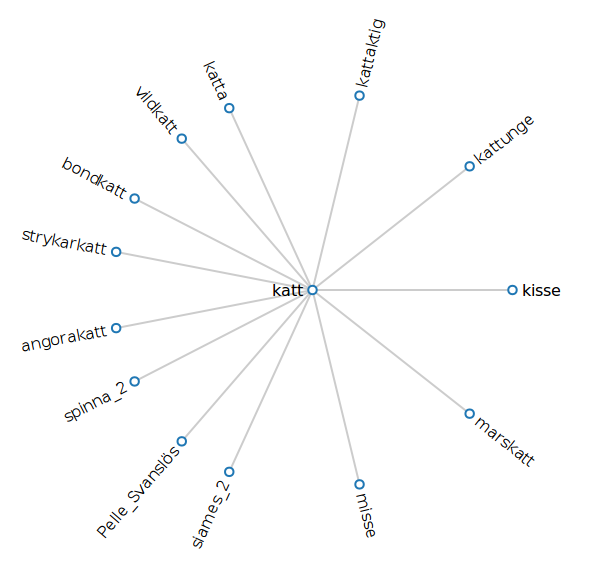
\includegraphics[width=60mm]{saldograph.png}
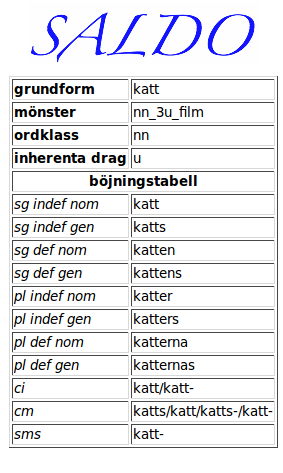
\includegraphics[width=40mm]{saldotab.png}
%What is saldo \\
%picture\\
% why it's hard (396 hur och hur)
%goals
\end{frame}


\begin{frame}[containsverbatim]
\frametitle{A large-scale lexicon}
\framesubtitle{} 
GF lexicons are generated by smart paradigms: \\
\vspace{5mm}
\begin{tabular}{ll}
\textbf{Regular verb} & \verb-mkV "hittar"- \\
\textbf{Irregular verb} &  \verb-mkV "knyter" "knöt" "knutit"- \\
\end{tabular}
\end{frame}

\begin{frame}
\frametitle{Importing Saldo}
\framesubtitle{Results} 
\begin{tabular}{ll}
Plural tantum nouns & Irregular s-verbs \\
\emph{glasögon} & \emph{umgås}\\
\end{tabular}\\
\vspace{5mm}
\begin{tabular}{ll}
\textbf{Result:} & Over 100 000 entries\\
\pause
&$\sim$500 missing words in Talbanken\\
\end{tabular}
\end{frame}

\begin{frame}
\frametitle{Grammar}
\framesubtitle{Swedish} 
\begin{tabular}{llll}
\textbf{Topicalization}& && \textbf{Passive}\\
Jag äter äpplet nu && &Äpplet blir ätet av mig \\
Äpplet äter jag nu &&& Äpplet äts av mig \\
\emph{``I eat the apple now"}& &&\emph{``The apple is eaten by me"}\\
%Nu äter jag äpplet &  & Jag äter sitt äpple \\
\end{tabular}
\end{frame}

\begin{frame}
\frametitle{Grammar}
\framesubtitle{Swedish} 
\begin{tabular}{lll}
 \textbf{Future tense}  &&\textbf{Impersonal constructions} \\
Jag ska sova nu & &Det bor två barn i huset \\
\emph{``I will sleep now"} && \emph{``There are two children living in the house"} \\
Jag kommer somna snart &&Det dansas på borden  \\
\emph{``I will fall asleep soon"} &&\emph{``People are dancing on the tables"}  \\
\end{tabular}
\end{frame}

\begin{frame}
\frametitle{Grammar}
\framesubtitle{Swedish} 
\textbf{Reflexive possessives prononus}\\
\begin{tabular}{lll}
Jag äter mitt äpple && Jag äter mitt äpple \\
\emph{``I eat my apple"} && \emph{``I eat my apple"} \\
Han äter sitt äpple && Han äter hans äpple \\
\emph{``He eats his apple"} && \emph{``He eats his apple"} \\
\end{tabular}
\end{frame}

%START OF DEMO
\begin{frame}
\frametitle{The grammar}
\framesubtitle{} 
\begin{tabular}{ll}
\textbf{Aim}: & Implement constructions frequent in Talbanken\\
&Restrict overgeneration\\
\end{tabular}\\
%intersting examples
%relate to gullmarsstrand
Passive\\
Formal subjects\\
Topicalisation - with particles, prepositions\\
Genitives \\
Reflexives
\end{frame}

%\begin{frame}
% \renewcommand{\baselinestretch}{1.5}
%\frametitle{The grammar}
%\framesubtitle{Current work} 
%\begin{tabular}{ll}
%\alert{\textbf{ReflGenVP}} & \alert{VPSlash $\rightarrow$ ReflCN $\rightarrow$ VP} \\
%& \alert{\emph{han ger sina små barn till dem}} \\
%{\textbf{PassVP}} & V2 $\rightarrow$ VP \\%  (should be VPSlash $\rightarrow$ VP) \\
%& \emph{äpplet åts} \\ % \;
%\alert{\textbf{AdvVPSlash}} & \alert{VPSlash $\rightarrow$ Adv $\rightarrow$ VPSlash} \\
%& \alert{\emph{hon åt redan äpplet}, \emph{hon är redan här}}\\
%\alert{\textbf{PPartAP}} & \alert{V2 $\rightarrow$ AP} \\
%& \alert{\emph{det är skrivet},\emph{den skrivna artikeln}}
%\end{tabular}\\
%\end{frame}

%\begin{frame}
%\frametitle{The grammar}
%\framesubtitle{Current work} 
%\begin{tabular}{ll}
%\alert{\textbf{ReflGenVP}} & \alert{VPSlash $\rightarrow$ ReflCN $\rightarrow$ VP} \\
%& \alert{\emph{han ger sina små barn till dem}} \\
%
% %\emph{("äpplet blev ätet")}\\ % boken gavs till honom
%\alert{\textbf{PassVP}}
%  & \alert{V2 $\rightarrow$ VP} \\ % (should be VPSlash $\rightarrow$ VP)} \\
%& \alert{\emph{äpplet åts},}\alert{\emph{boken gavs till honom}} \\ 
%
%% CompAdv here, plus we need ComlVVAdv, Pass? osv
%\alert{\textbf{AdvVPSlash}} & \alert{VPSlash $\rightarrow$ Adv $\rightarrow$ VPSlash} \\
%& \alert{\emph{hon åt redan äpplet}, \emph{hon är redan här}}\\
%% &\emph{("hon åt äpplet redan")} \\
%
%\textbf{PPartAP} & V2 $\rightarrow$ AP \\
%& \emph{det är skrivet},\emph{den skrivna artikeln}
%\end{tabular}\\
%\pause
%%Easy sentences with known words (old testsuite) : 92 out of 118 (78\%) \\
%%list of functions
%%examples
%%difficulties
%%sådan
%\end{frame}

\begin{frame}
 \renewcommand{\baselinestretch}{1.0}
\frametitle{Evaluation}
\framesubtitle{} 
Reached aims\\
Some nice results\\
Discussions\\
\end{frame}




\begin{frame}
\frametitle{Mapping}
\framesubtitle{Example} 
\small{\textbf{Talbanken05}}\hspace{160pt}
\small{\textbf{GF abstract tree}}
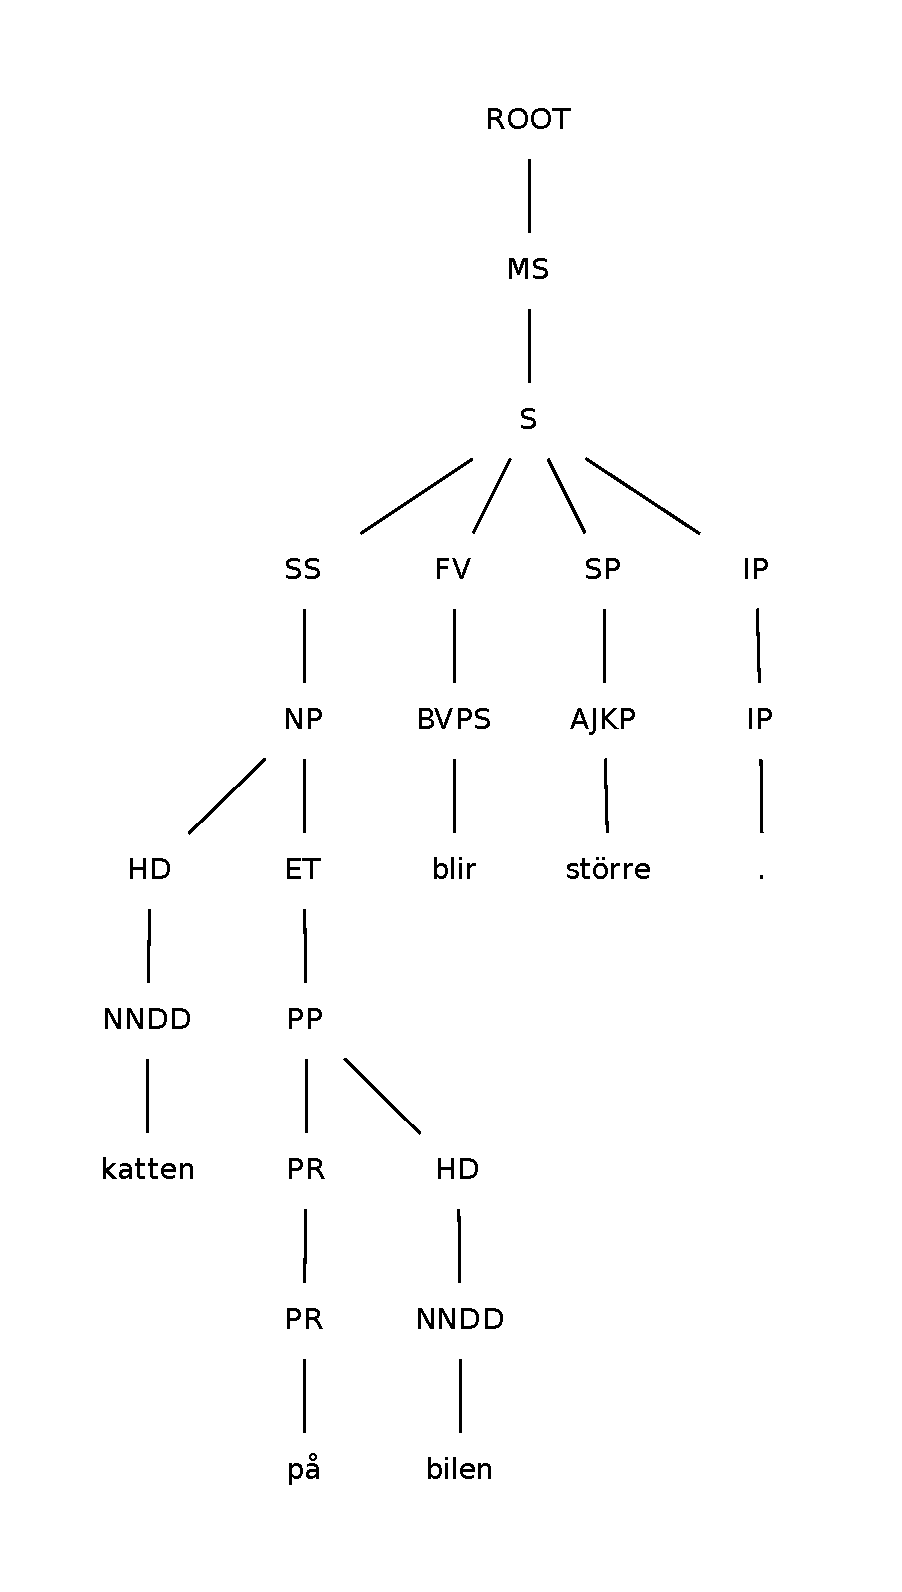
\includegraphics[width=130pt,height=200pt]{taltree.pdf}
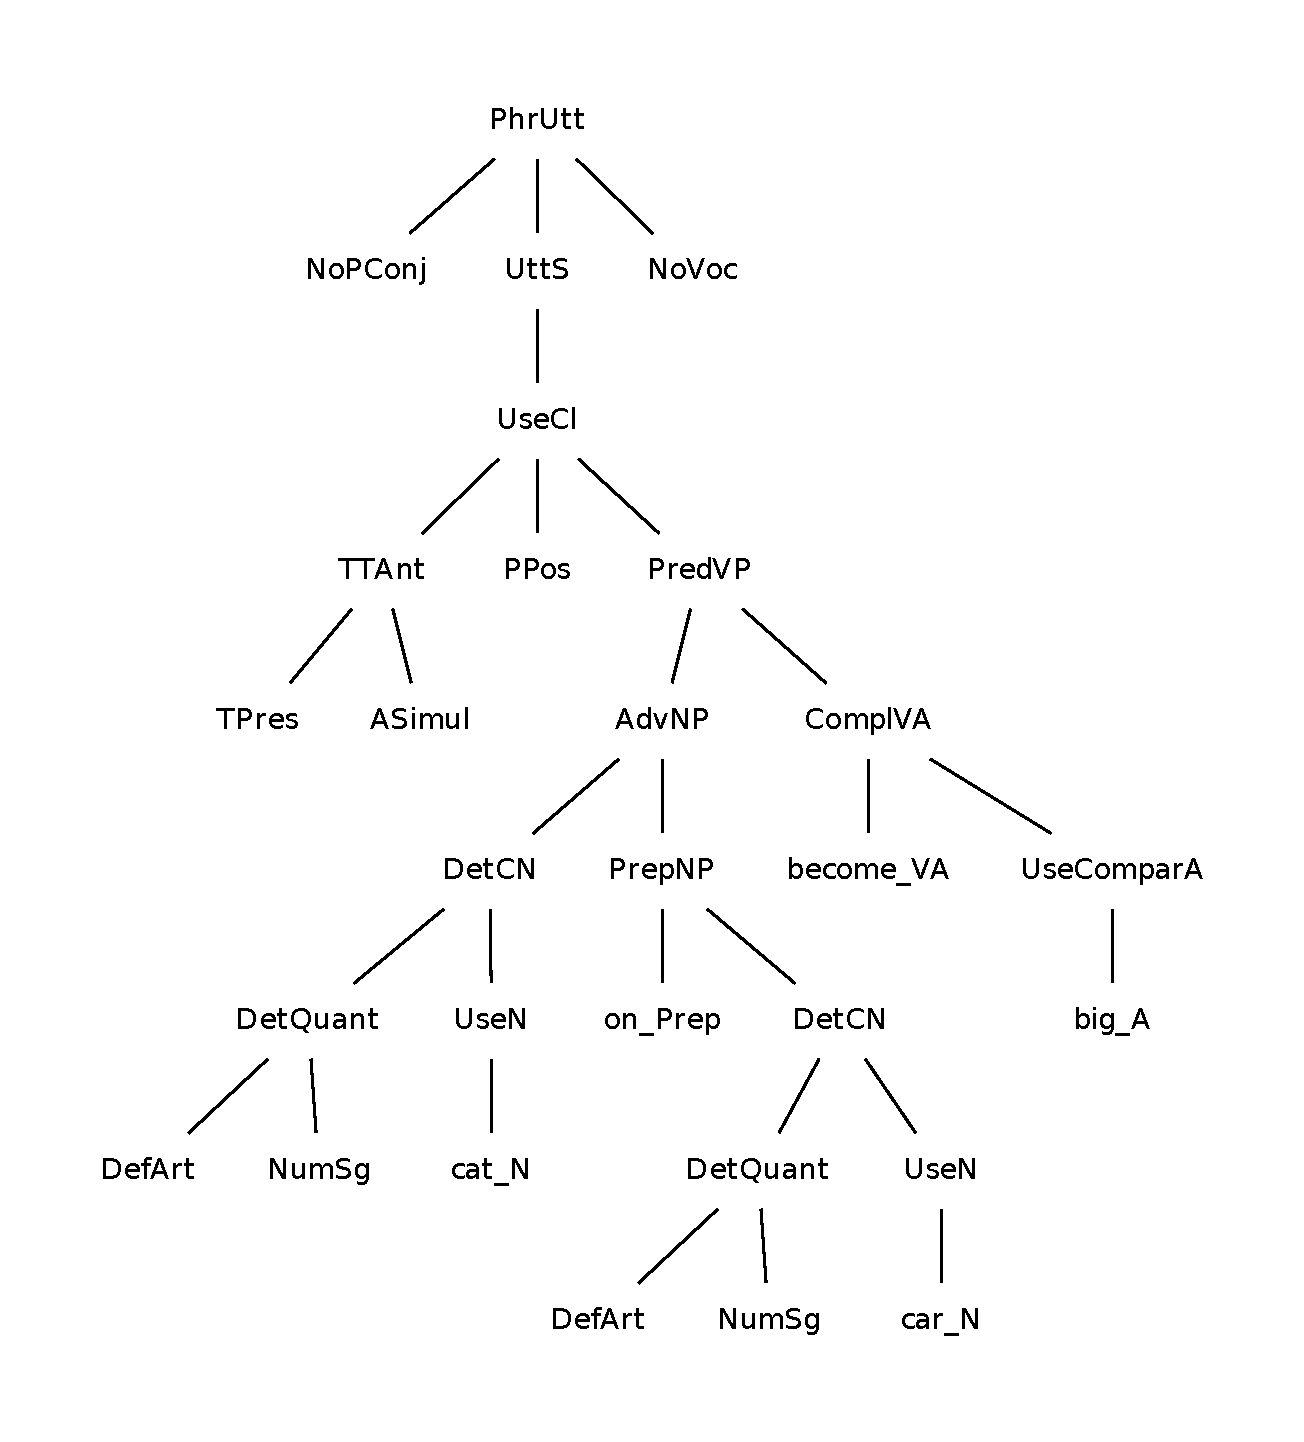
\includegraphics[width=170pt,height=200pt]{gftree.pdf}
\end{frame}




\begin{frame}
 \renewcommand{\baselinestretch}{1.0}
\frametitle{}
\framesubtitle{Future work} 
Lexicon
Probabilitis
Chunk parsing
\end{frame}

\begin{frame}
    \frametitle{The end}
\large\begin{center}Thanks for listening\end{center}
\end{frame}
\end{document}

